\section{Terminal}
\subsection{Vue Terminal}
\par Cette vue terminal permet d'afficher le modèle dans le terminal, néanmoins cela reste toujours plus lent qu'une implémentation sur une interface graphique, ce pourquoi il est conseillé de privilégier la vue via l'interface.
\begin{figure}[H]
        \center
        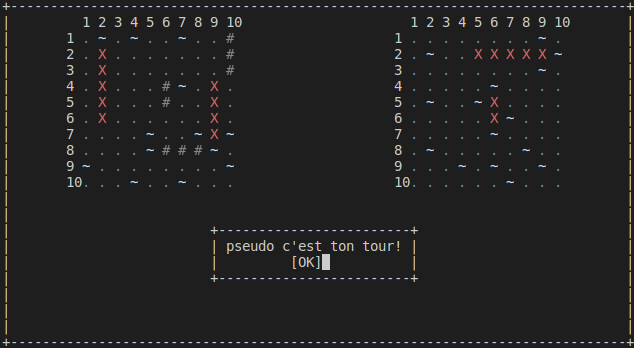
\includegraphics[scale=0.5]{images/terminal/PartieEnCours.png}
        \caption{Interface utilisateur en début de partie dans le terminal}
\end{figure}

\par Les bateaux de l'interface sont représentés par des \textbf{\#} gris, l'eau est représenté par des \textbf{.} bleus, les coups manqués par des \textbf{$\sim$} blancs (sensé représenter les vagues causées par un tir dans l'eau) et les tirs touchés sont représentés par des \textbf{X} rouges. L'affichage terminal a aussi un mode d'affichage "caché" qui cache les bateaux tant qu'ils ne sont pas touchés.

\subsection{Contrôleur Terminal}
Le contrôleur terminal va initialiser plusieurs choses avant de commencer la partie comme :\begin{itemize}
\item Le pseudo de l'utilisateur,
    \begin{figure}[htp]
        \centering
        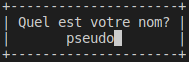
\includegraphics[scale=1]{images/terminal/ChoixNom.png}
        \caption{\label{fig: ChoixNomTe}Choix du pseudo}
    \end{figure}
\item La version de l'IA adverse (RandomPlayer ou IAPlayer),\\
    \begin{figure}[htp]
        \centering
        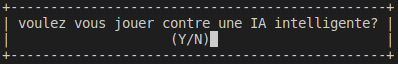
\includegraphics[scale=0.5]{images/terminal/ChoixAdversaire.png}
        \caption{\label{fig: ChoixAdversaireT}Choix de l'adversaire}
    \end{figure}
\item Le placement des bateaux.\\
    \begin{figure}[htp]
        \centering
        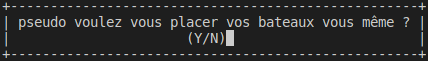
\includegraphics[scale=1]{images/terminal/ChoixPlacement.png}
        \caption{\label{fig: ChoixPlacementT}Choix du placement des bateaux}
    \end{figure}
\end{itemize}
\par Si le placement des bateaux est manuel, le joueur place ses bateaux en commençant par le plus grand le porte-avions long de 5 cases, suivi par le croiseur de 4 cases, 2 sous-marin de 3 cases et enfin le torpilleur de 2 cases.
\par Pour cela, le joueur devra rentrer les coordonnées d'une case, et dans quel sens se situe son bateau. Si le placement est correct (le bateau est intégralement dans la grille, ne se superpose pas avec un autre bateau, ni est adjacent à l'un d'entre eux), le bateau est placé et on continue avec le prochain, jusqu'à qu'ils soient tous placés.
\par Une fois cela fait, la partie peut commencer. Chaque joueur peuvent jouer un coup l'un après l'autre, et pour un joueur Humain il le fait en indiquant les coordonnées du coup souhaité, une à une.